% !TEX spellcheck = de_DE
% !TeX root = Vorlesung.tex
%---------------------------------------------------------------------------------
\section[Windenergiegewinnung]{Optimale Windenergiegewinnung}\label{sec:WEN}
%---------------------------------------------------------------------------------
\miniframesoff	
\begin{frame}<handout:0>[noframenumbering]{Inhalt}
\tableofcontents[currentsection]
\PutAt<1-|handout:0>[5cm]{(10cm,2cm)}{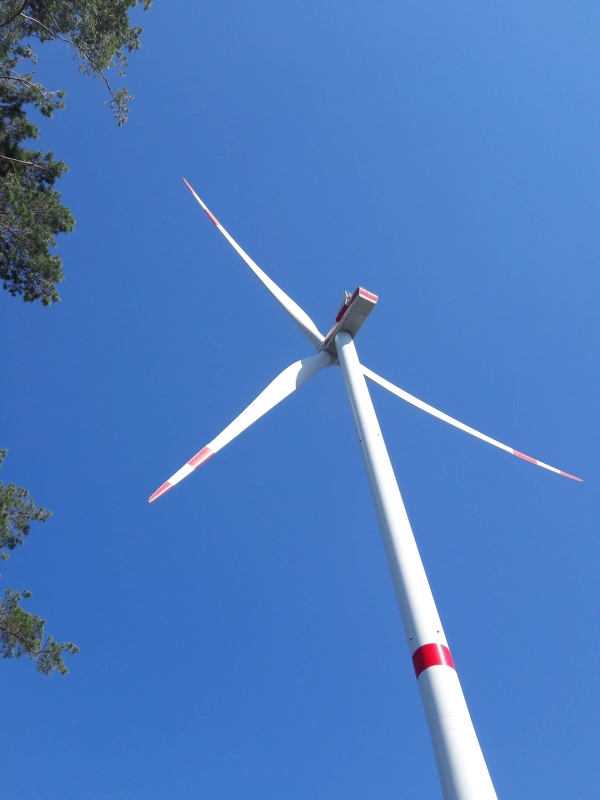
\includegraphics[width=4.0cm]{\StylePath/content/Fronrot}} % graphic related to topic	
\end{frame}
\miniframeson
%---------------------------------------------------------------------------------
\begin{frame}{Energie und Leistung des Windes} 
\setlength{\abovedisplayskip}{0pt}
\setlength{\belowdisplayskip}{0pt}
\begin{columns}
	\column{9cm} 
	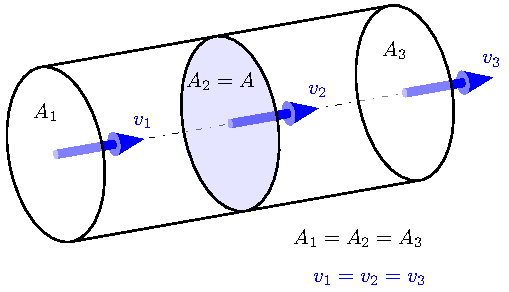
\includegraphics[width=\linewidth]{WEN/streamtube1.pdf}		
	\column{6cm}
	\vspace*{-1pt}
	\begin{block}<1->{Kinetische Energie}
		\begin{align*}
		E   & = \frac{1}{2} m v_1^2
		\end{align*}
		\begin{tabular}{ll}
			$m$ 	&  Luftmasse\\
			$v_1$ 	&  ungestörte Windgeschw.
		\end{tabular}
	\end{block}	
	%---
	\begin{block}<2->{Massenstrom}
		\begin{align*}
		\dot m & = \rho A v_1
		\end{align*}
		\begin{tabular}{ll}
			$\rho $ 	&  Luftdichte\\
			$A$ 		&  Kontrollfläche
		\end{tabular}	
	\end{block}	
	%---
	\begin{block}<3->{Leistung des Windes}
		\begin{align*}
		P_{\textnormal{Wind}}=\dot E = \frac{1}{2} \rho A v_1^3 
		\end{align*}
	\end{block}	
	%---	
\end{columns} 	
\end{frame}
%---------------------------------------------------------------------------------
\begin{frame}{Energieentnahme durch Abbremsen} 
\begin{figure}[htbp]
	\begin{center}
		\begin{minipage}[c]{0.4\linewidth}
			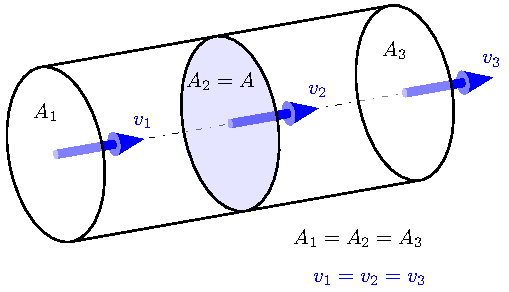
\includegraphics[width=\linewidth]{WEN/streamtube1.pdf}
		\end{minipage}
		\visible<2->{
			\begin{minipage}[c]{0.4\linewidth}
				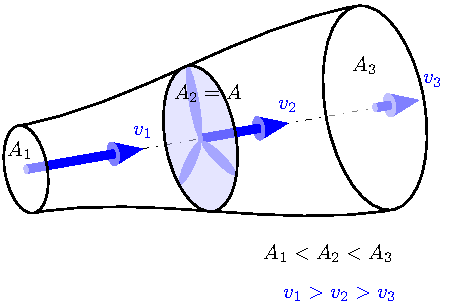
\includegraphics[width=\linewidth]{WEN/streamtube2.pdf}
			\end{minipage}
		}
		\begin{minipage}[c]{0.15\linewidth}
			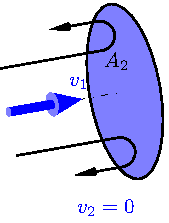
\includegraphics[width=\linewidth]{WEN/streamtube3.pdf}
		\end{minipage}
	\end{center}
\end{figure}
\begin{block}<1->{}
\begin{itemize}
	\item Energie kann dem Wind durch Abbremsung extrahiert werden (Windenergiekonverter)
	\item für die Betrachtung verwendet Betz eine stark idealisierte WEA ohne Verluste % cite!!!
	\item keine Energieentnahme ohne oder bei vollständiger Abbremsung 
	\item <2-> Optimum muss dazwischen liegen!
	\item <2-> Stromröhre aus Kontinuitätsgründen: $\rho A_1 v_1= \rho A_2 v_2= \rho A_3 v_3$
\end{itemize}
\end{block}	 
\end{frame}
%---------------------------------------------------------------------------------
\begin{frame}{Pioniere der Windenergie-Entwicklung} 
\begin{columns}
	\column{7cm}
	\centering
	\includegraphics<1->[height=4.8cm,trim=0 9.25cm 0 0, clip] {WEN/Hau2014Fig2.17}
	\begin{columns}
		\column{3.0cm} 		
		\begin{block}<2->{}{Wasserstoff aus Windstrom}\end{block}	
		\column{3.0cm} 
		\begin{block}<2->{}{Betz'sches Gesetz, Blattdesign}\end{block}	
	\end{columns}	
	\column{7cm}
	\centering
	\includegraphics<3->[height=4.8cm,trim=0 0 0 9.25cm, clip] {WEN/Hau2014Fig2.17}
	\begin{columns}
		\column{3.0cm} 
		\begin{block}<4->{}{Erste MW Windturbine}\end{block}	
		\column{3.0cm} 
		\begin{block}<4->{}{Blätter aus Verbundstoffen}\end{block}		
	\end{columns}		
\end{columns} 
\flushright\tiny\textcolor{gray}{\cite{Hau2014}}	
\end{frame}		 		 
%---------------------------------------------------------------------------------
\begin{frame}{Maximaler Leistungsbeiwert nach Betz} 
\setlength{\abovedisplayskip}{0pt}
\setlength{\belowdisplayskip}{1pt}
\begin{columns}
\column{8cm}
	%---	
	\begin{block}<1->{Entnommene Energie}
		\begin{align*}
		E   & = \frac{1}{2} m v_1^2 - \frac{1}{2} m v_3^2 = \frac{1}{2} m (v_1^2 - v_3^2)
		\end{align*}
	\end{block}	
	%---	
	\vspace*{-1pt}
	%---
	\begin{block}<2->{Entnommene Leistung}
		\begin{align*}
		P   & = \frac{1}{2} \dot m (v_1^2 - v_3^2) \quad\textnormal{mit}\quad v_2=\frac{v_1+v_3}{2}\\
		& = \underbrace{\frac{1}{2}\rho Av_1^3}_{P_{\textnormal{Wind}}}
		\underbrace{\frac{1}{2}\left(1+\frac{v_3}{v_1}\right)\left(1-\left(\frac{v_3}{v_1}\right)^2\right)}_{c_{\textnormal{P}}}
		\end{align*}
	\end{block}	
	%---	
	\vspace*{-1pt}
	%---	
	\begin{block}<3->{Leistungsbeiwert $c_{\textnormal{P}}$ und Induktionsfaktor $a$}
		\begin{align*}
		c_{\textnormal{P}} = \frac{P}{P_{\textnormal{Wind}}} = 4a(1-a)^2 \quad\textnormal{mit}\quad 1-a=\frac{v_2}{v_1}
		\end{align*}
	\end{block}	
	%---
	%---	
\column{6cm} 
	\centering
	\includegraphics<3->[width=6cm] {WEN/BetzOptimum.pdf}
	\begin{block}<3->{}
		Maximum: $c_{\textnormal{P}}=\frac{16}{27}$ bei $\frac{v_3}{v_1}=\frac{1}{3}$ und $a=\frac{1}{3}$
	\end{block}			
\end{columns} 
\end{frame}
%---------------------------------------------------------------------------------
\begin{frame}{Maximaler Leistungsbeiwert nach Betz } 
\setlength{\abovedisplayskip}{0pt}
\setlength{\belowdisplayskip}{1pt}
	\begin{block}<1->{Leistungskoeffizient $c_{\textnormal{P}}$}
		\begin{align*}
			c_{\textnormal{P}} & = \frac{P}{P_{\textnormal{Wind}}} = \frac{1}{2} \left( 1 + \frac{v_3}{v_1} \right) \left( 1 - \left( \frac{v_3}{v_1} \right)^2 \right) \text{\ mit\ } x=\frac{v_3}{v_1}\\
			& = \frac{1}{2} (1+x)(1-x^2)=\frac{1}{2}(-x^3-x^2+x+1)
		\end{align*}
	\end{block}	
	%---	
	\vspace*{-1pt}
	%---
	\begin{block}<2->{Ableitung von $c_{\textnormal{P}}$}
		\begin{align*}
		c_{\textnormal{P}}' &= \frac{\textnormal{d} c_{\textnormal{P}}}{\textnormal{d}x} = \frac{1}{2} \left( - 3 x^2 - 2 x +1 \right)\overset{!}{=}  0 \quad \Rightarrow \quad x=\frac{v_3}{v_1} = \frac{1}{3}
		\end{align*}
	\end{block}
	%---	
	\vspace*{-1pt}
	%---
	\begin{block}<3->{Maximum von $c_{\textnormal{P}}$}
		\begin{align*}
		c_{\textnormal{P}} \left( \frac{v_3}{v_1} = \frac{1}{3} \right) &= \frac{1}{2} \left( 1 + \frac{1}{3} \right) \left( 1 - \left( \frac{1}{3} \right)^2 \right) = \frac{16}{27} \approx 59\%
		\end{align*}
	\end{block}
\end{frame}
%---------------------------------------------------------------------------------
\begin{frame}{Schubbeiwert nach Betz}
\setlength{\abovedisplayskip}{0pt}
\setlength{\belowdisplayskip}{1pt} 	
\begin{columns}
\column{8cm}
	%---	
	\begin{block}<1->{Schubkraft (Thrust $T$)}
		\begin{align*}
		T   &= \dot m  (v_1 - v_3)  \quad\textnormal{mit}\quad v_2=\frac{v_1+v_3}{2}\\
		&= \underbrace{\frac{1}{2}\rho v_1^2}_{\textnormal{dynamischer Druck}} A 
		\underbrace{\left(1-\left(\frac{v_3}{v_1}\right)^2\right)}_{c_{\textnormal{T} } }
		\end{align*}
	\end{block}	
	%---	
	\begin{block}<2->{Schubbeiwert $c_{\textnormal{T}}$ und Induktionsfaktor $a$}
		\begin{align*}
		c_{\textnormal{T}} = 4a(1-a) \quad\textnormal{with}\quad 1-a=\frac{v_2}{v_1}
		\end{align*}
	\end{block}	
	%---
	%---	
\column{6cm} 
	\centering
	\visible<3>{
	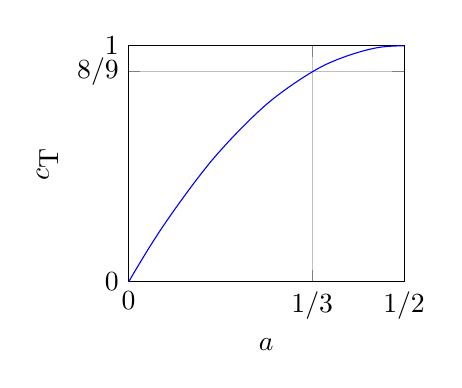
\begin{tikzpicture}
	\begin{axis}[x=7cm,y=3cm,grid=major, xmin=0, xmax=0.5, ymin=0, ymax=1, xlabel=$a$, 
	ylabel=$c_{\textnormal{T}}$,
	ytick={0,8/9,1},
	xtick={0,1/3,0.5},
	yticklabels={0,8/9,1},
	xticklabels={0,1/3,1/2}
	]
	\plot[blue] plot[samples=100, smooth] expression{4*x*(1- x)};
	\end{axis}	
	\end{tikzpicture}
	}
	\begin{block}<3->{}
		\begin{itemize}
			\item $c_{\textnormal{T}}=\frac{8}{9}$ bei $a=\frac{1}{3}$
			\item 	$c_{\textnormal{T}}\approx1.1$ für eine runde Scheibe\\
			\item[$\rightarrow$] im optimalen Fall ähnelt der Schub dem einer festen Scheibe
		\end{itemize}	
	\end{block}			
\end{columns} 
\end{frame}
%---------------------------------------------------------------------------------
\begin{frame}{Theorem von Froude und Rankine}
\setlength{\abovedisplayskip}{0pt}
\setlength{\belowdisplayskip}{1pt} 
\begin{columns}
	\column{5.8cm} 
	\centering
	\includegraphics<1->[width=5.8cm] {WEN/Gasch2012Fig5.5.pdf}\\	
	\flushright\tiny\textcolor{gray}{\cite{Gasch2016}}	
	\column{8.2cm}
	\begin{block}<1->{Theorem}
		\begin{align*}
	 		v_2=\frac{v_1+v_3}{2}
		\end{align*}
	\end{block}		
	\begin{block}<1->{Schritte der Herleitung}
		\begin{itemize}
			\item Schub $T$ als Impulsänderungsdifferenz ausdrücken: $T=\dot{m}(v_1-v_3)$.\\
			\item Bernoulli-Gleichung für Bereich unmittelbar vor und hinter dem Rotor anwenden.\\
			\item Anwendung von $v_{-2}=v_{+2}$ (Kontinuitätsgleichung) und $p_1=p_3$ führt zu $\frac{\rho}{2} \left( v_1^2-v_3^2 \right) = p_{-2}-p_{+2}$.\\
			\item Schub als Druckdifferenz ausdrücken $T=A(p_{-2}-p_{+2})$ und $\dot{m}=\rho A v_2$ anwenden.
		\end{itemize}
	\end{block}	
\end{columns} 	
\end{frame}
%---------------------------------------------------------------------------------
\begin{frame}{Grundkonzepte von Windenergiekonvertern} 
\begin{columns}
	\column{9.0cm} 
		\centering
		\includegraphics<1->[width=9cm] {WEN/Gasch2016Fig3.1.pdf}\\	
		\flushright\tiny\textcolor{gray}{\cite{Gasch2016}}	
	\column{5.0cm}
	\begin{block}<1->{Moderne Windturbinen}
		\begin{itemize}
		\item Auftriebsläufer, horizontal und Luvläufer
		\item 3-blättrig: bester Kompromiss zwischen Last, Energie und Kosten
		\item die besten Anlagen erreichen $c_{\textnormal{P}}=52\%$
		\item Schnelllaufzahl $\lambda=\frac{v_{\textnormal{tip}}}{v_1}$ normalerweise um \num{7}
		\item Widerstandsläufer werden als Anemometer verwendet, üblich $c_{\textnormal{P}}=10\%$
		\end{itemize}
	\end{block}	
\end{columns} 	
\end{frame}
%---------------------------------------------------------------------------------